\chapter{Восстановление треков в дрейфовых камерах}
Выбор дрейфовых камер в качестве координатных детекторов спектрометра на
экспериментальной установке СТРЕЛА обусловлен возможностью получения высокого
пространственного разрешения и более надёжного отбора двух близко проходящих
треков частиц.

Применение дрейфовых камер требует нахождения соотношения между измеренным
временем дрейфа проходящей частицы и его преобразованием в расстояние
относительно данной сигнальной проволочки. Сначала используется <<интегральное>>
преобразование, после чего происходит поиск и реконструкция трека. Для получения
более корректного соотношения между временем дрейфа и расстоянием используется
итеративная процедура автокалибровки.

\section{Время дрейфа, TDC}
Временной спектр TDC одного из каналов показан на рис.~\ref{fig:tdc}.
Минимальное и максимальное время дрейфа ($T_{min},\,T_{max}$) для каждого канала
(проволочки) определяется аппроксимацией его временного спектра функцией
\begin{equation}
  \label{eq:tdc_fit}
  N(t) = p[2] + p[3]\,erfc\,\Biggl[\frac{(t - p[0])}{\sqrt{2}\,p[1]} \Biggr]\,,
\end{equation}
отдельно для минимального времени, $T_{min} = p[0] + p[1]$, и отдельно для
максимального, $T_{max} = p[0]$. $erfc(x)$~--- дополнительная функция
ошибок~\cite{erfc_web}. Параметры $p[2]$ и $p[3]$ можно использовать для
качественной проверки фита. Среднее полное время дрейфа составляет
$\sim$~450~нс.

\begin{figure}[h]
  \centering
  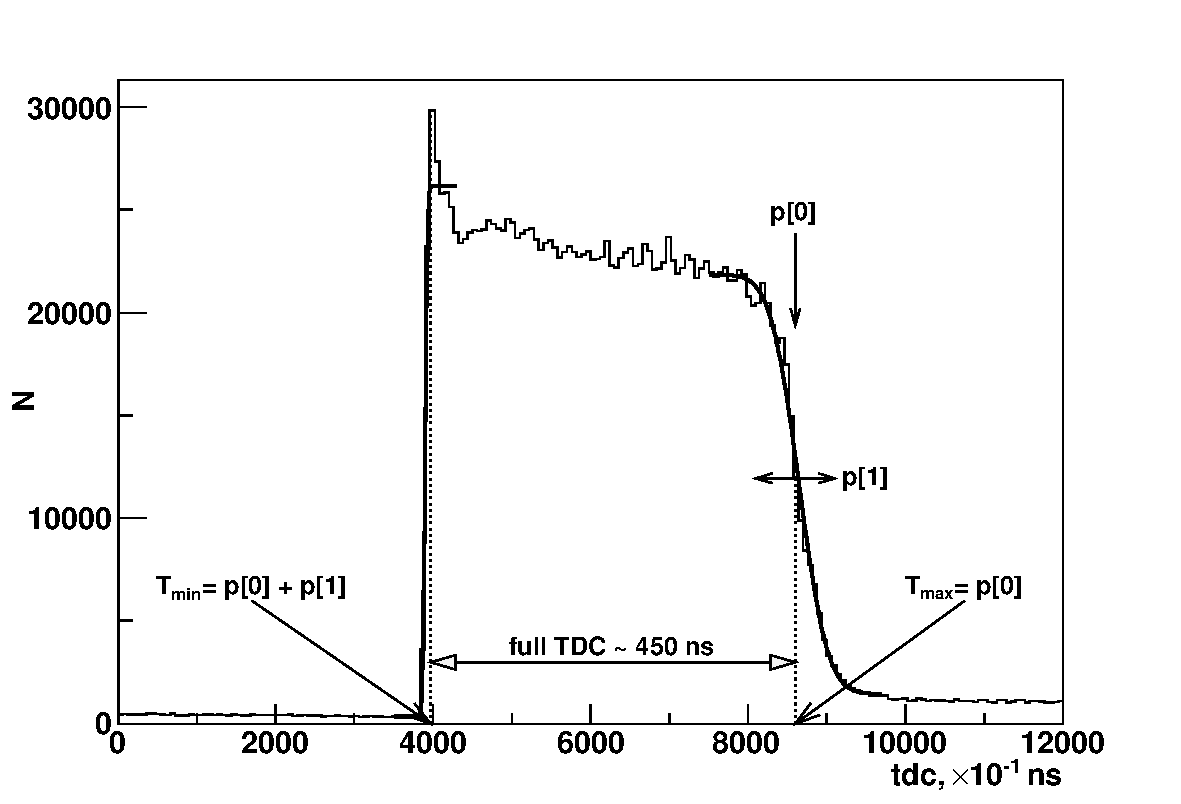
\includegraphics[width=1.00\textwidth]{tdc.pdf}
  \caption{Временной спектр $TDC$ одного из каналов (проволочек) дрейфовой
    камеры. Сплошные линии~--- аппроксимация распределения в области
    минимального $T_{min}$ и максимального $T_{max}$ времени
    функцией~\eqref{eq:tdc_fit}.}
  \label{fig:tdc}
\end{figure}

Соотношение между измеренным временем дрейфа и минимальным расстоянием между
анодной проволочкой и треком частицы имеет важнейшую роль при реконструкции
трека в дрейфовых камерах. Задача состоит в определении функции преобразования
времени дрейфа $t$ в расстояние $r$, так называемое $r(t)$-отношение, зависящее
от многих параметров: напряжённости электрического поля, состава газовой смеси,
давления, температуры, геометрии дрейфовой камеры~\cite{pesehonov86}.

Если предположить, что поток падающих частиц является равномерным, а
эффективность во всей области чувствительности проволочки постоянна, то скорость
дрейфа можно выразить как
\begin{equation}
  v_{d}(t) = \frac{dr}{dt} = \frac{dr}{dN}\,\frac{dN}{dt} =
  const\,\frac{dN}{dt}\,, \qquad
  const = \frac{dr}{dN} = \frac{R}{N_{tot}}\,,
\end{equation}
где $R$~--- длина дрейфового промежутка (21~мм), $N_{tot}$~--- полное число
событий и $dN/dt$~--- временное распределение (рис.~\ref{fig:tdc}).

Таким образом, функцию преобразования времени дрейфа $t$ в расстояние $r$ можно
выразить как
\begin{equation}
  r(t) = \int_{T_{min}}^{T_{max}} v_{d}(t')\,dt' = \frac{R}{N_{tot}}
  \int_{T_{min}}^{T_{max}} \frac{dN}{dt'}\,dt'\,.
\end{equation}
Заметим, что так полученное $r(t)$-отношение (рис.~\ref{fig:t2r}) будет
корректироваться (поправляться) в итеративном процессе
автокалибровки~\cite{gla_mucha10}.

\begin{figure}[h]
  \centering
  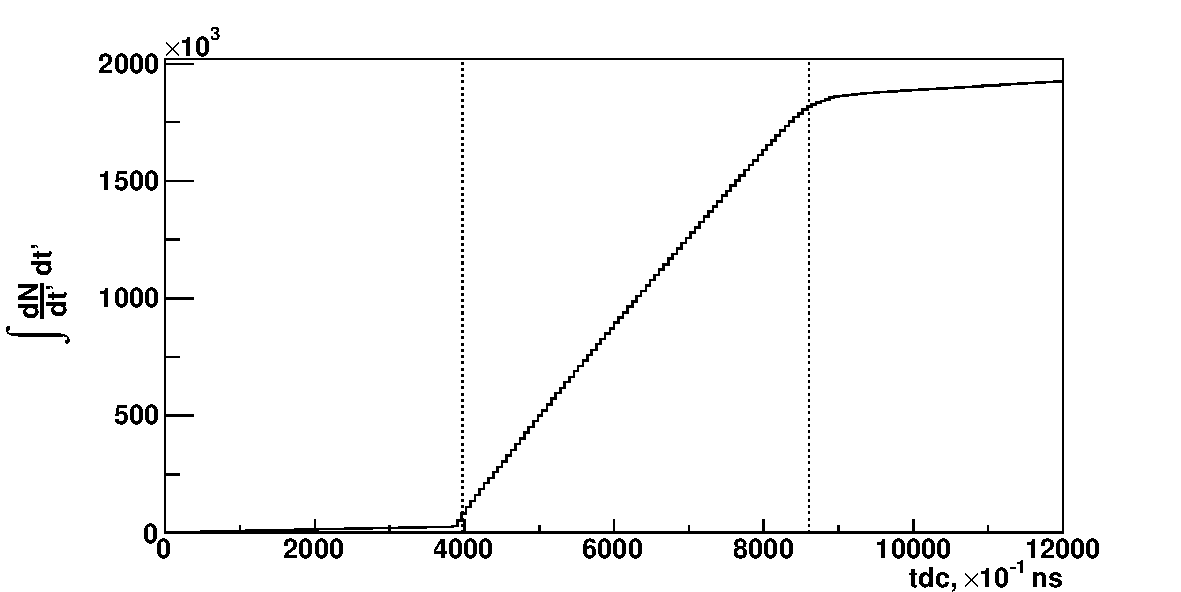
\includegraphics[width=0.965\textwidth]{t2r_t.pdf}
  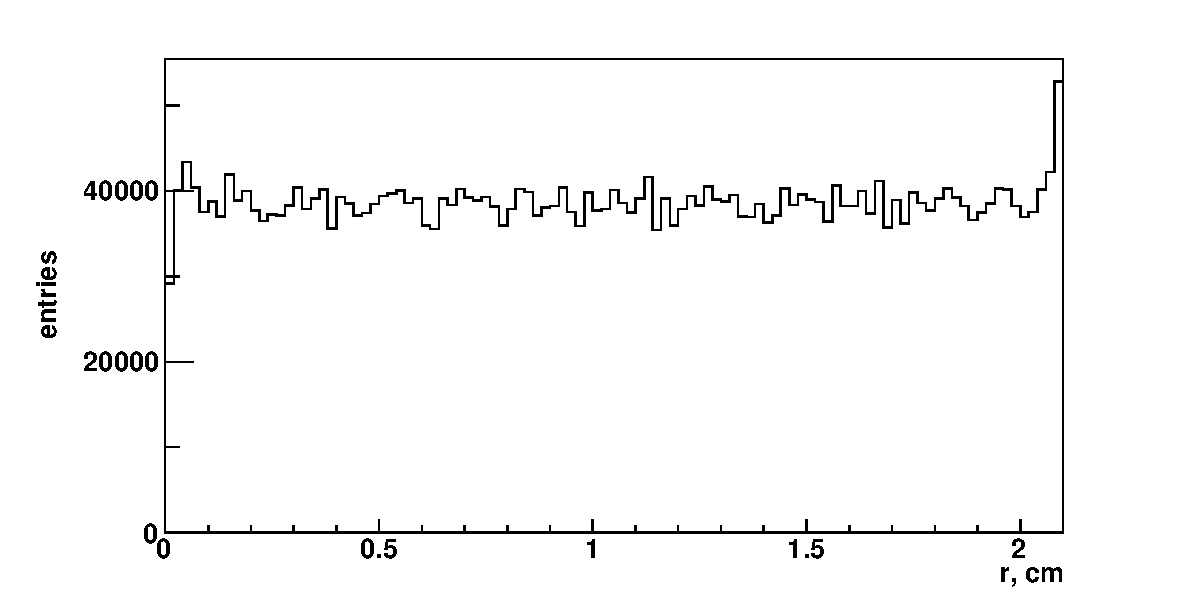
\includegraphics[width=0.965\textwidth]{t2r_r.pdf}
  \caption{На верхнем рисунке интегрированное время дрейфа $t$ проволочки из
    рис~\ref{fig:tdc}. Нижний рисунок~--- преобразованное расстояние $r$ между
    проволочкой и треком.}
  \label{fig:t2r}
\end{figure}

\section{Поиск трека}
Поиск (а позднее и реконструкция) трека происходит отдельно для каждого блока
дрейфовых камер одной плоскости $xz$ или $yz$-координат. В зависимости от
конкретной задачи, можно программным путём, соединять (или разделять) блоки
камер в один мультиблок. В одном блоке (или мультиблоке) должно быть не менее
трёх слоев сигнальных проволочек, для возможности однозначного определения
трека.

\begin{figure}[h]
  \centering
  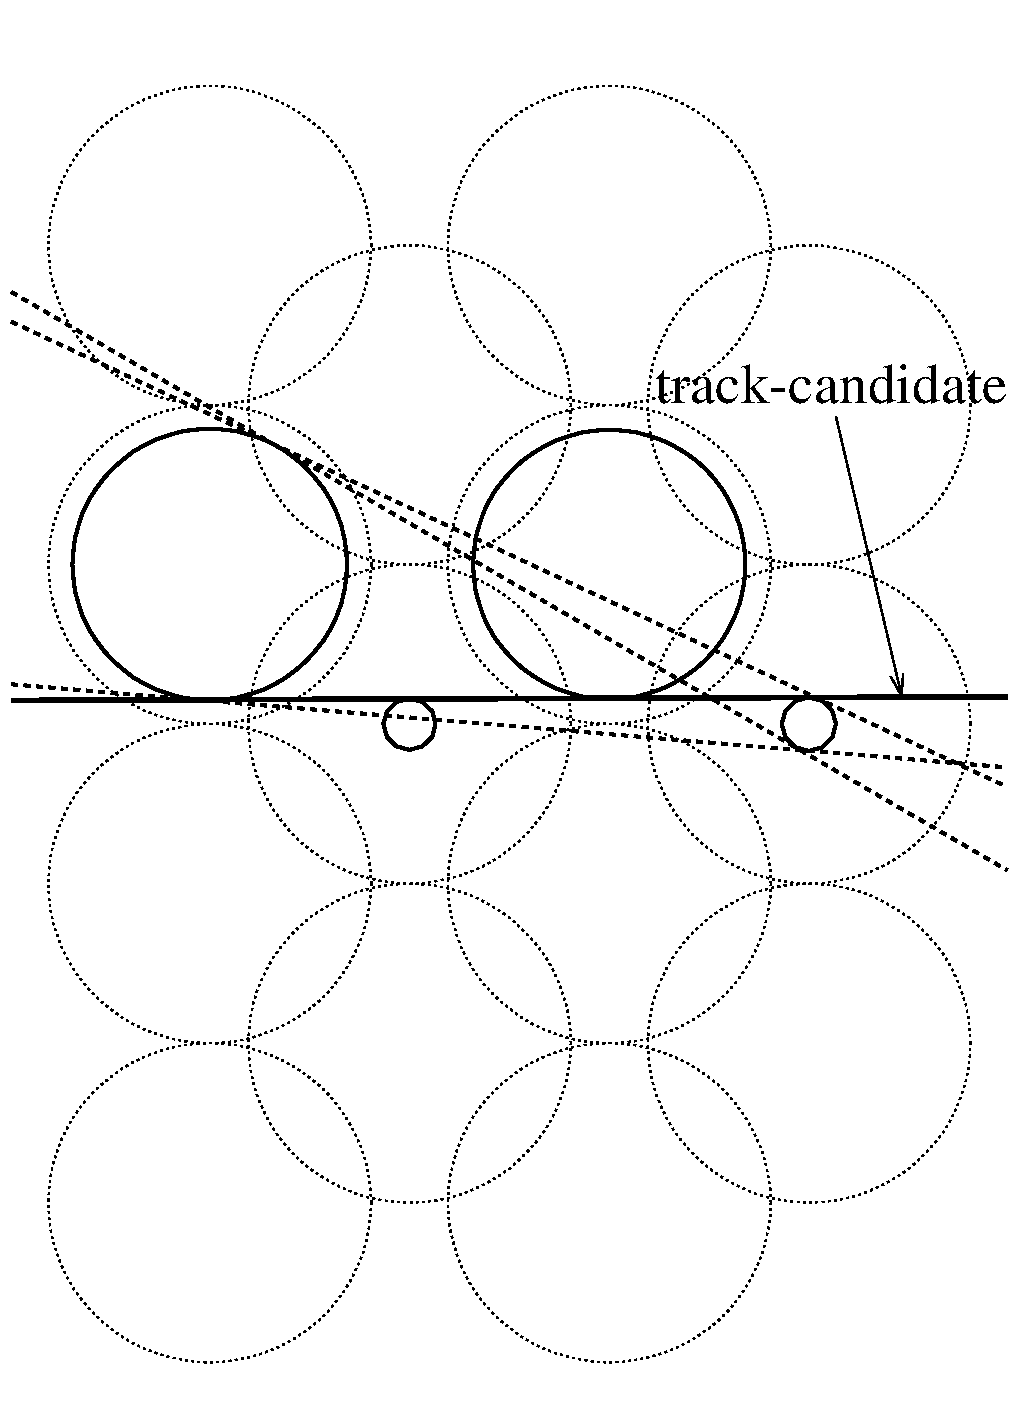
\includegraphics[width=0.48\textwidth]{event_112_run126.pdf} \hfill
  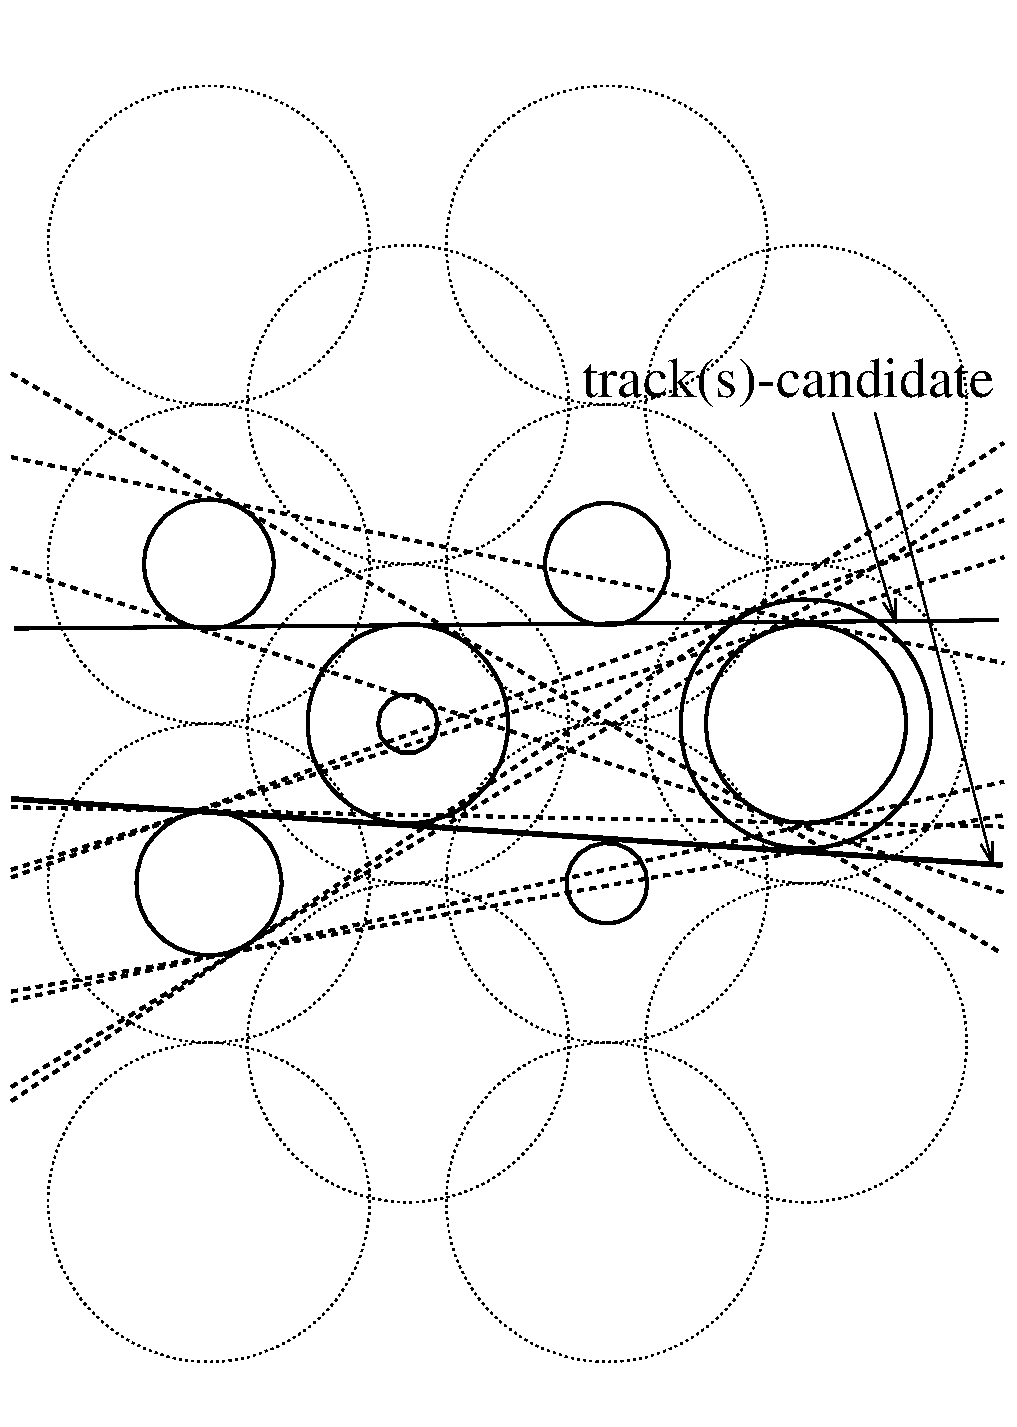
\includegraphics[width=0.48\textwidth]{event_104_run126.pdf}
  \caption{Пример проекции однотрекового (влево) и двухтрекового (вправо)
    события в одной плоскости блока первой дрейфовой камеры, состоящей из
    четырёх слоёв проволочек. Штриховые окружности представляют максимальную
    длину дрейфового промежутка, сплошные~--- расстояние трека от сигнальной
    нити. Для визуального изображения дрейфового промежутка используются
    окружности, центры которых проходят через сигнальные проволочки.}
  \label{fig:typo_2events}
\end{figure}

Последовательность поиска трека в упрощённом виде можно изложить следующим
образом:
\begin{enumerate}
\item Поиск пары сработавших проволочек из разных слоев камеры, имеющих
  наибольшее расстояние. Для пары окружностей, представляющих расстояние
  проекции трека от сигнальной нити, вычисляются параметры всех четырёх
  касательных, рис.~\ref{fig:typo_2events}.
\item Для каждой касательной вычисляется её расстояние $d$ от окружности
  сработавших проволочек. Если расстояние больше, чем заданное минимальное
  $d > d_{min}$, то сработавшая проволочка отбрасывается (не считается).
  $d_{min}$ обычно на порядок больше, чем пространственное разрешение камеры.
\item Если число сработавших проволочек $N_{hits}$ камеры, удовлетворяющих
  предыдущему условию, для касательной не менее заданного
  $N_{hits} \geq  N_{min}$, то касательная переходит в разряд кандидатов в трек.
  Для нашего примера (рис.~\ref{fig:typo_2events}) $N_{min}$ равно 4. Если
  кандидатов несколько, то оставляется тот, у которого сумма расстояний $d$
  минимальна.
\item Производится реконструкция трека и возвращение к 1.~пункту, т.е. поиску
  последующей пары в данном блоке дрейфовой камеры. Сработавшие проволочки,
  которые вошли  в восстановленный трек, не удаляются, и их можно использовать
  для поиска и реконструкции следующего трека.
\end{enumerate}

\section{Реконструкция трека}
Полученный трек-кандидат используется в процедуре реконструкции, восстановления
трека. Проекцию прямого трека в плоскости перпендикулярной к проволочкам блока
дрейфовой камеры можно параметризовать как уравнение прямой
\begin{equation}
  X = aZ + b
\end{equation}
с параметрами $a$ и $b$, рис.~\ref{fig:reco_scheme}.

\begin{figure}[h]
  \centering
  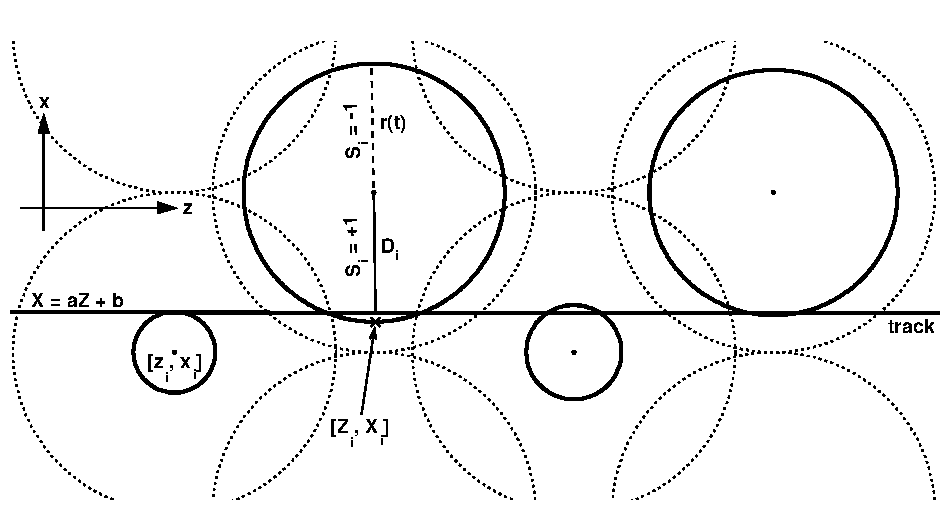
\includegraphics[width=1.00\textwidth]{event_137_run126.pdf}
  \caption{Определение параметров используемых при реконструкции трека в
    блоке дрейфовой камеры.}
  \label{fig:reco_scheme}
\end{figure}

Предположим, что трек имеет $N$ сработавших проволочек с координатами
$(z_i, x_i)$ для $i = 1, \ldots N$. Тогда расстояние между треком и $i$-й
проволочкой можно выразить как
\begin{equation}
  D_i = \frac{a z_i - x_i + b}{\sqrt{1 + a^{2}}}\,.
\end{equation}

Задача реконструкции трека состоит в получении параметров прямой $a$ и $b$
путём минимизации $\chi^2$-функции
\begin{equation}
  \label{eq:chi2_1}
  \chi^2 = \frac{1}{N-2}\sum_{i=1}^{N} [|D_i| -S_ir_i]^2 =
  \frac{1}{N-2}\sum_{i=1}^{N} \biggl[
    \Big|\frac{az_i - x_i + b}{\sqrt{1 + a^2}}\Big| - S_ir_i\biggr]^2\,,
\end{equation}
где $S_i$ имеет в зависимости от положения трека относительно проволочки
значение $\pm{1}$ (рис.~\ref{fig:reco_scheme}), $r_i$~--- расстояние между
треком и $i$-й проволочкой, полученное из функции преобразования времени дрейфа
$t$ в расстояние $r$. Величины параметров $a$ и $b$ получаем решением двух
дифференциальных уравнений
$\frac{\partial \chi^2}{\partial a} = 0$ и
$\frac{\partial \chi^2}{\partial b} = 0$, которые можно решить итеративно.
Уравнение~\eqref{eq:chi2_1} можно переписать следующим образом
\begin{equation}
  \label{eq:chi2_2}
  \chi^2 = \frac{1}{N-2}\sum_{i=1}^{N}
  \biggl[\frac{aZ_i - X_i + b}{\sqrt{1 + a^2}}\biggr]^2\,,
\end{equation}
где координаты проволочек $(z_i, x_i)$ заменяем координатами $(Z_i, X_i)$,
которые вычисляются как
\begin{equation}
  \label{eq:chi2_3}
  Z_i = z_i - S_ir_i \frac{a_0}{\sqrt{1 + a_0^2}}\,, \qquad
  X_i = x_i + S_ir_i \frac{1}{\sqrt{1 + a_0^2}}\,.
\end{equation}

Минимизируя $\chi^2$-функцию (уравнение~\eqref{eq:chi2_2}) методом наименьших
квадратов, получаем значения трековых параметров $a$ и $b$ в виде
\begin{equation}
  a = \frac{-\,\beta + \sqrt{\,\beta^{\,2} + 4\,\alpha^2}}{2\,\alpha}\,, \qquad
  b = S_X - a\,S_Z\,,
\end{equation}
где
\begin{equation}
  \alpha = S_{ZX} - S_Z\,S_X\,, \qquad
  \beta = S_{ZZ} - S_{XX} - S_Z^2 + S_X^2
\end{equation}
и
\begin{equation}
  \begin{split}
    S_Z = \sum_{i=1}^{N} Z_i\,, \qquad
    S_X = \sum_{i=1}^{N} X_i\,, \qquad
    S_{ZX} = \sum_{i=1}^{N} Z_i \, X_i\,, \\
    S_{ZZ} = \sum_{i=1}^{N} Z_i^2\,, \qquad
    S_{XX} = \sum_{i=1}^{N} X_i^2\,. \qquad \qquad \\
  \end{split}
\end{equation}
Величину $a_0$ в итеративном процессе последовательно заменяем новым значением
$a$. В качестве начального значение $a_0$ в уравнении \eqref{eq:chi2_3}
используем параметр $a$ из трека-кандидата (касательной). Для частиц падающих
на камеру под небольшими углами можно принять $a_0 = 0$.

В среднем, после двух--трёх итераций параметры $a$ и $b$ практически не
меняются, и если значение $\chi^2/ndf$ меньше заданного, то трек считаем
восстановленным.

\section{Процедура автокалибровки}
Для реконструкции треков необходимо знать отношение между измеренным временем
дрейфа и его преобразованием в расстояние, поэтому получение правильного
$r(t)$-отношения, является одной из важнейших задач. Итеративную процедуру
определения $r(t)$-отношения с использованием трековой информации называем
автокалибровкой~\cite{bac97,pet05,ame04}.

Отметим, что $r(t)$-отношение, полученное в процессе равномерного облучения
частицами дрейфового промежутка не учитывает неравномерность напряжённости
электрического поля вдоль траектории дрейфа электронов, а это, в свою очередь,
приводит к изменению величины скорости дрейфа, и соответственно, к
дифференциальной нелинейности $r(t)$-отношения. Это возможно в конструкции
используемых дрейфовых камер, где напряжённость электрического поля вдоль
траектории дрейфа задаётся резистивной сборкой, резисторы которой имеет разброс
в несколько процентов.

Однако можно предположить приблизительно одинаковые условия в камере, для
которой выполняется автокалибровка. При необходимости можно программным путём
разделить камеры на меньшие или на группы проволочек, для которых предполагаем
те же самые условия. Иногда поиск и реконструкция трека происходит в одном
блоке (мультиблоке) камер, но процедура автокалибровки проделывается для
каждой камеры отдельно.

\begin{figure}[!h]
  \centering
  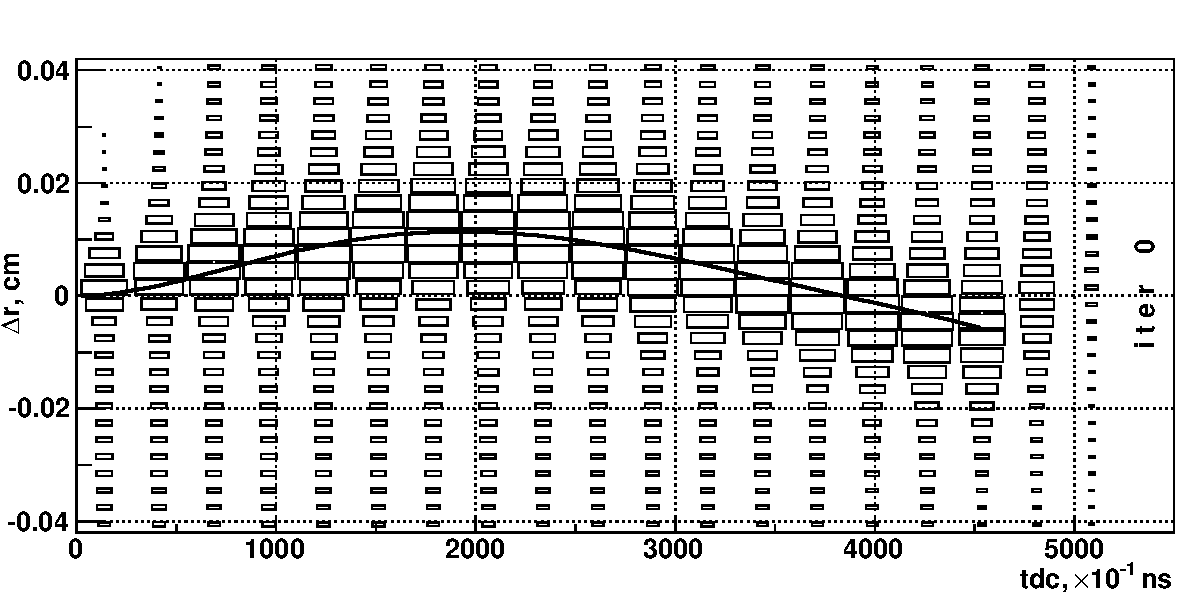
\includegraphics[width=1.00\textwidth]{multi_iter0.pdf}
  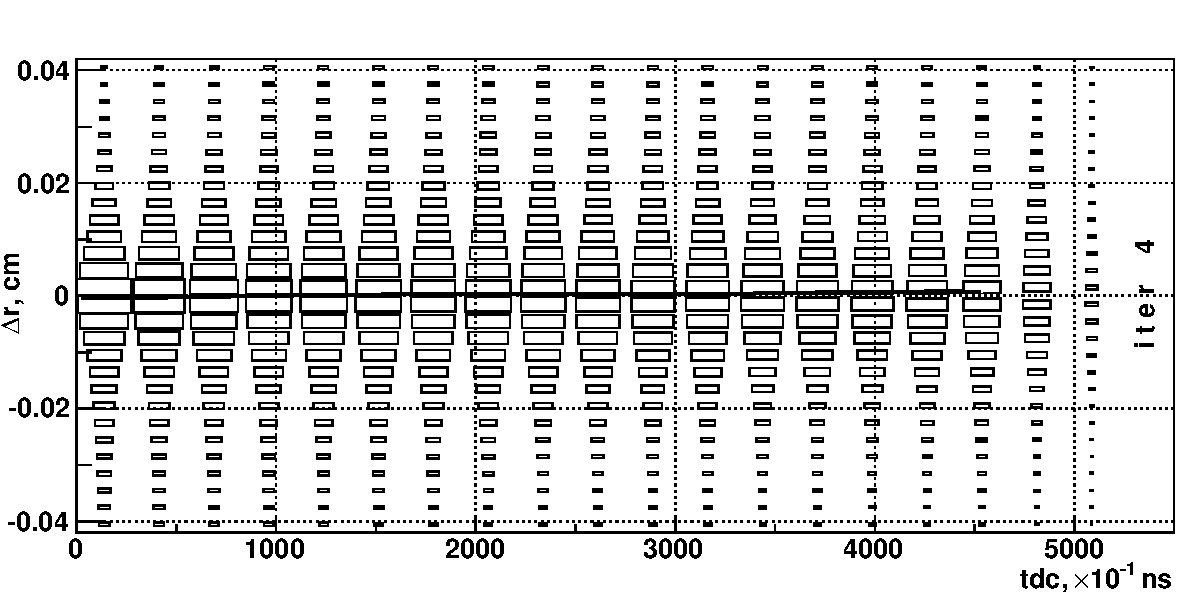
\includegraphics[width=1.00\textwidth]{multi_iter4.pdf}
  \caption{Зависимость распределения трекового остатка $\triangle r$ от времени
    дрейфа $t$ в одной плоскости блока больших дрейфовых камер. Верхний
    рисунок~--- исходное $r(t)$-отношения (интегральное преобразование времени
    в расстояние), нижний рисунок~--- после окончательной, четвёртой итерации
    автокалибровки. Размер прямоугольника пропорционален числу событий. Сплошная
    линия~--- аппроксимация средних значений трекового остатка для каждого
    временного интервала.}
  \label{fig:multi_iter}
\end{figure}

На рис.~\ref{fig:multi_iter} показана зависимость трекового остатка
$\triangle r$ (residual) от времени дрейфа в блоке большой дрейфовой камере.
Трековый остаток можно определить как
\begin{equation}
  \triangle r = r - |D|\,,
\end{equation}
где $r$~--- расстояние полученное преобразованием ($r(t)$-отношение) времени
дрейфа $t$, а $D$~--- расстояние восстановленного трека от проволочки.

Распределение трекового остатка (его ширина) в основном определяется
пространственным разрешением дрейфовой камеры. Тем не менее, $\triangle r$
можно использовать при решении таких задач, как юстирование, сбалансирование
проволочек в блоках (мультиблоках) камер относительно друг друга или для
дополнительной оценки минимального и максимального времени дрейфа. Ожидаемое
среднее значение трекового остатка $\triangle r \simeq 0$.

По горизонтальной оси двумерной зависимости распределения $\triangle r$ от $t$
(рис.~\ref{fig:multi_iter}) отложено время дрейфа с шагом гистограммы 27.5~нс.
Шаг выбран так, чтобы получить необходимое число временных интервалов. В нашем
примере оно равно 20. Для каждого временного интервала создаётся проекция
трекового остатка $\triangle r$. Полученные распределения остатков
аппроксимируются распределением Гаусса, среднее значение которого представляет
поправку $\delta_i$ к текущему $r(t)$-отношению в каждом $i$-м временном
интервале. Таким образом, получается новая, подправленная функция преобразования
времени дрейфа $t$ в расстояние $r$, с которой вновь выполняется реконструкция
трека.

В каждом следующем шаге процедуры автокалибровки $r(t)$-отно\-шение поправляется
в зависимости от предыдущей итерации. Поиск и реконструкция треков проводится
повторно до тех пор, пока значения поправок $\delta_i$ для всех временных
интервалов стабилизируются (приблизятся к нулевым значениям). В нашем примере
число итераций равно 4--5. Как меняется распределение трекового остатка в
зависимости от номера итерации, показано на рис.~\ref{fig:per_iterative}.
Видно, что с ростом номера итерации трековый остаток стремится к нулю, а ширина
распределения уменьшается.

\begin{figure}[h]
  \centering
  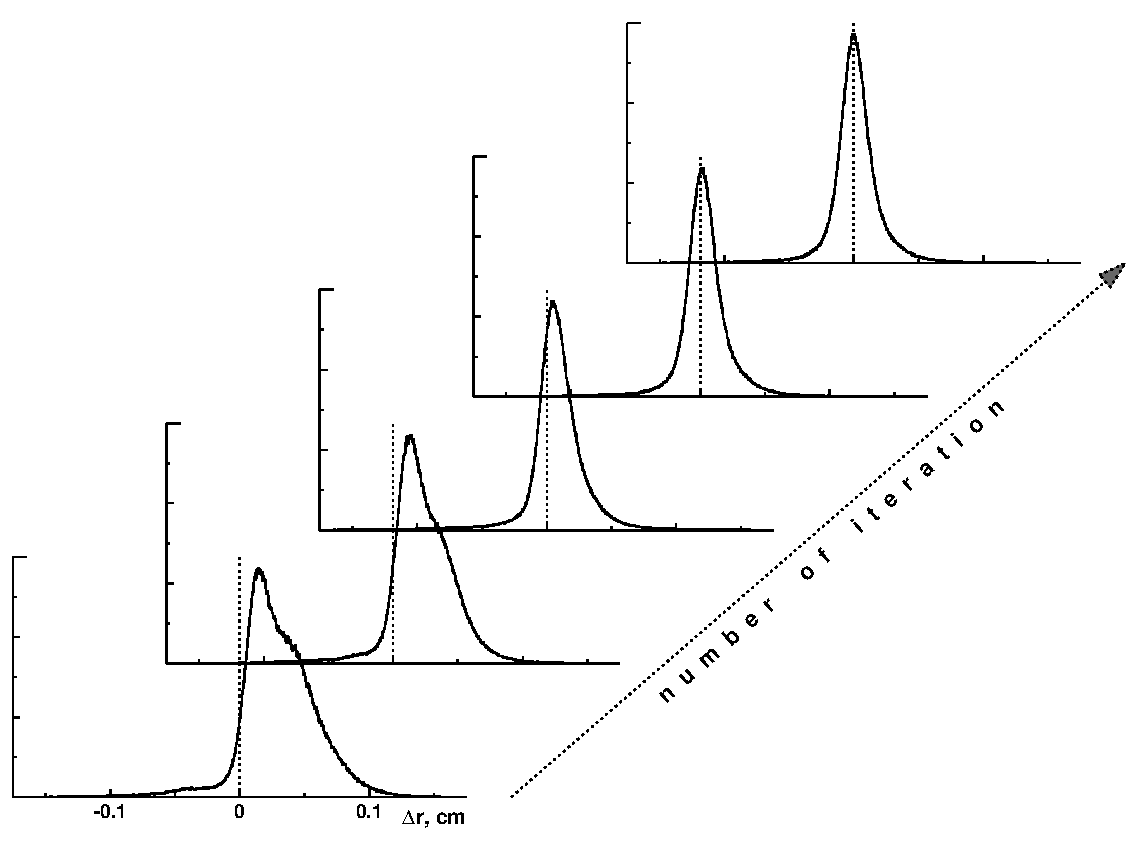
\includegraphics[width=1.00\textwidth]{c_per_iterative.pdf}
  \caption{Изменение распределения трекового остатка $\triangle r$ в зависимости
    от номера итерации в блоке больших дрейфовых камер.}
  \label{fig:per_iterative}
\end{figure}

Процесс автокалибровки выполняется только с однотрековыми событиями. Желательно,
чтобы угловой разброс треков в камере не превышал $\sim$~100~мрад. Если диапазон
наклонов треков, проходящих через камеру, большой, то итеративную процедуру
автокалибровки делаем отдельно для разных диапазонов углов наклона. Область
изменения угла наклона не должна превышать
$\sim$~100--150~мрад~\cite{gla_mucha08_2}.

Пространственное разрешение дрейфовой камеры определяется шириной распределения
трекового остатка данной камеры. Для вычисления разрешения $\sigma$
использовалась аппроксимация двойным распределением Гаусса,
рис.~\ref{fig:res_chambers}. Пространственное разрешение дрейфовых камер,
используемых на установке СТРЕЛА, лежит в диапазоне $\sim$~90--120~мкм.
Влиянием многократного рассеяния (дейтроны с импульсом 3.5 ГэВ/с) на разрешение
можно пренебречь.

\begin{figure}[!h]
  \centering
  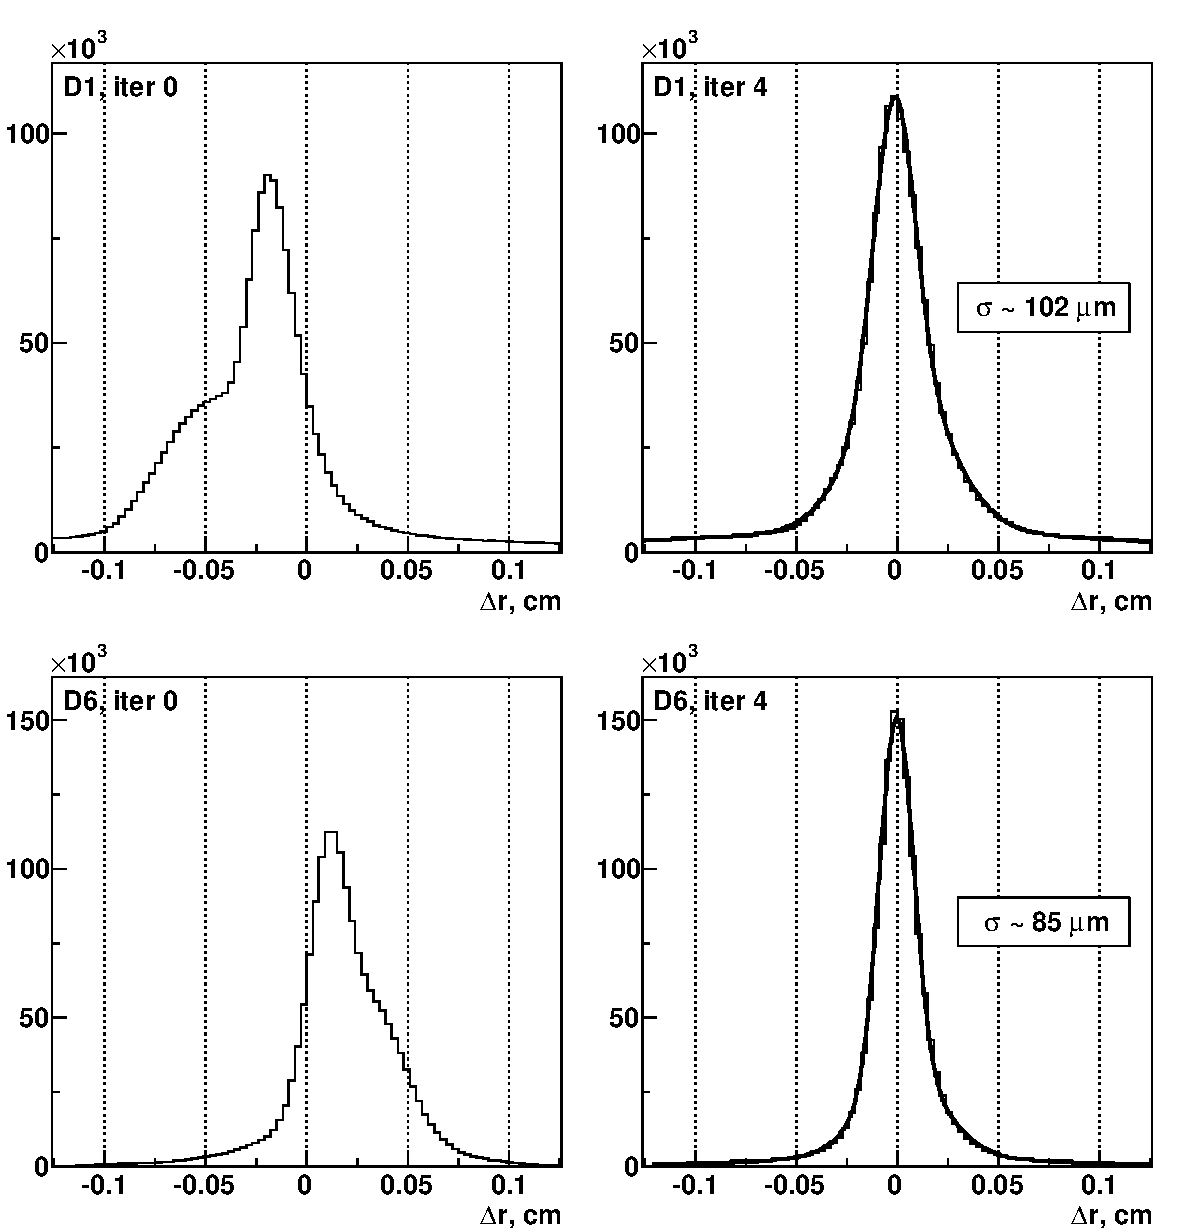
\includegraphics[width=1.00\textwidth]{res_chambers.pdf}
  \caption{Распределения трекового остатка $\triangle r$ в $xz$-плоскости
    дрейфовой камеры D1 и камеры D6. Слева~--- распределения с исходным
    интегральным $r(t)$-отношением, справа~--- после финальной четвёртой
    итерации автокалибровки, аппроксимированные двойным распределением Гаусса.}
  \label{fig:res_chambers}
\end{figure}

\section{Выводы к четвёртой главе}
Из проведённого в этой главе анализа можно сформулировать основные результаты:
\begin{list}{\labelitemi}{\leftmargin=1em}
\item В процессе создания и усовершенствования установки СТРЕЛА был разработан
  и реализован полный комплекс программ обработки и анализа экспериментальных
  данных.
\item Разработаны и протестированы на реальных событиях алгоритмы для поиска и
  реконструкции треков в дрейфовых камерах. Исходный код программ написан
  полностью на языке С++ с использованием библиотек ROOT, что делает их
  универсальными и модульными.
\item Показано, что созданная итеративная процедура автокалибровки существенно
  улучшает величину пространственного разрешения камер, среднее значение которой
  лежит в диапазоне 90--120~мкм.
\item Полученные характеристики трековых детекторов позволяют осуществить
  исследования зарядово-обменных процессов в дейтрон-протонных взаимодействиях
  на установке СТРЕЛА.
\item Созданная нами методика реконструкции событий после небольших изменений
  может быть использована и для других экспериментов, где применяются
  координатные детекторы, такие как дрейфовые камеры или трубки.
\end{list}

%%% Local Variables:
%%% mode: latex
%%% TeX-master: "musinsky_disser"
%%% coding: utf-8
%%% End:
